\chapter{Intro to ML}


\section{ML Problem Formulation}

\textbf{Input}: \\
Let $x$ be the input, where $x\in\mathcal{X}\subset\mathcal{D}$. In practical applications, this input could be in various forms such as a piece of text, an image, an audio clip, or data from a sensor output.\\


\textbf{Output}: \\
The output is denoted as $\mathbf{y}$, where $\mathbf{y}\in\mathcal{Y}$. $\mathcal{Y}$ is the set of all possible outputs This is typically a label or a predicted outcome based on the given input.\\

\textbf{Experience \(\mathcal{X}\)}: \\
This refers to the observations or the training data set that falls within domain \(D\). The data points are denoted as \(x \in \mathcal{X} \subseteq D\). The pairs \((x_1, y_1), (x_n, y_n)\) denote the individual data and target output points.\\


\textbf{Target Function $f:\mathcal{X}\to\mathcal{Y}$}: \\
The target function is denoted as $f$ which maps from $\mathcal{X}$ to $\mathcal{Y}$, represented as $f:\mathcal{X}\to\mathcal{Y}$. In real-world scenarios, this true underlying function is never known in practice.\\

\textbf{Domain of Data $\mathcal{D}$}: \\
The set of all possible data points for testing or out-of-sample validation. It is represented as \(D\). Data is the fundamental component used to train models in machine learning. It is often represented as a set of input-output pairs: $(\mathbf{x}_1,y_1),(\mathbf{x}_n,y_n),\ldots,(\mathbf{x}_n,y_n)$. \\

\textbf{Error Function $\widehat{R}_n$}: \\
The error function quantifies the deviation of the predicted output from the actual output. It's represented as:
\[
\widehat{R}_n=\frac1n\sum_n\widehat{l}(g(w,x),y)
\]\\

In machine learning, the symbol $\hat{l}$ usually refers to the \textbf{estimated loss} or \textbf{empirical loss}. It quantifies how well a particular model's predictions match the true data.\\

\begin{itemize}
    \item \textbf{Purpose}: The purpose of $\hat{l}$ is to evaluate the performance of a model on a dataset. A lower empirical loss indicates that the model is making fewer errors on that specific dataset.
    
    \item \textbf{Usage}: It is used in various algorithms to adjust model parameters in order to minimize this loss, thereby improving the model's predictions.
    
    \item \textbf{Difference from True Loss}: It's important to note the distinction between empirical loss and the true loss. While the empirical loss is computed using the training data, the true loss measures the expected loss over the entire distribution of data, which is typically unknown.
    
    \item \textbf{Overfitting Concern}: Relying solely on $\hat{l}$ can lead to overfitting if the model becomes too tailored to the training data and loses its generalisation ability for unseen data.
\end{itemize}

By carefully choosing and sometimes regularising the empirical loss function, practitioners can guide the learning algorithm to produce models that generalise well to new, unseen data.


\section{Machine Learning Components}

\begin{definitionbox}{Expertise}
This encompasses the models and predictors utilised in the learning process. The main objective is to formulate a hypothesis \(g: \mathcal{X} \rightarrow \mathcal{Y}\) that closely approximates the target function.
\end{definitionbox}

\begin{definitionbox}{Learning}
The process by which the hypothesis class \( \mathcal{H} \subseteq \{ h: \mathcal{X} \rightarrow \mathcal{Y} \} \) is refined using a specific learning algorithm to achieve the goal \(g \approx f\).
\end{definitionbox}

\begin{definitionbox}{Error \(g \approx f\)}
The difference between the hypothesis \(g\) and the target function \(f\). It can be quantified using various error functions and metrics such as \( l: (g, \mathcal{Y}) \rightarrow \mathbb{R}^+ \) and \( R_n = \frac{1}{n} \sum_{i=1}^{n} |g(w,x) - f(x)| \).
\end{definitionbox}

\begin{examplebox}{Problem Formulation for the Wine Quality Dataset}


\begin{tabular}{|l|l|l|l|}
\hline
\textbf{Data Set Characteristics}  & Multivariate               & \textbf{Instances Count}  & 4898 \\ \hline
\textbf{Attribute Characteristics} & Real                       & \textbf{Attributes Count} & 12   \\ \hline
\textbf{Tasks}                     & Regression, Classification & \textbf{Missing Values?}  & N/A  \\ \hline
\end{tabular}



\begin{itemize}
    \item Two datasets were created, using red and white wine samples
    \item The output is based on sensory data, rating 0-10 by experts
\end{itemize}


\textbf{Attributes}
\begin{enumerate}[nolistsep]
    \item fixed acidity
    \item volatile acidity
    \item citric acid
    \item residual sugar
    \item chlorides
    \item free sulfur dioxide
    \item total sulfur dioxide
    \item density
    \item pH
    \item sulphates
    \item alcohol
    \item quality (score between 0 and 10)
\end{enumerate} 
\vspace{\baselineskip}
\textbf{Domain:} $\mathcal{D}\subset\{\mathbf{x}:\mathbf{x}\in\mathbb{R}^{11}\}$

\textbf{Data Samples:} $X\subset\mathcal{D},\mathbf{x}_n\in\mathbb{R}^{11}, n=1, \ldots N=4898$

\textbf{Target Function:} $f:X\to\mathcal{Y},f(x)=y,x\in\mathcal{X},y\in\mathbb{R},y\in[1,10]$

\textbf{Hypothesis Class:} \( \mathcal{H} \subseteq \{ h: \mathcal{X} \rightarrow \mathcal{Y} \} \)

\textbf{Error Function:} $\widehat{R} = \text{Mean Squared Error (MSE)} = \frac{1}{n} \sum_{i=1}^{n} (y_i - \hat{y}_i)^2$ 

Note: $y_i$ is the actual quality score and $\hat{y}$ us the predicted quality score
\end{examplebox}

\section{Analysis of a Simple Hypothesis Class}

\subsection{Overview}
A hypothesis class defines a set of possible functions that can be learned given a set of data. The slide discusses a linear predictor, which attempts to predict outputs based on a linear combination of the inputs.

\subsection{Inputs and Model Parameters}
\begin{itemize}
    \item \textbf{Input,} $x$: This is a vector of numerical values, $(x_1, \dots, x_d)$, which represent the features or attributes of the data.
    \item \textbf{Model Parameters,} $w$: These are weights corresponding to each input feature, represented as $(w_1, \dots, w_d)$. The weights dictate the importance of each feature in the linear combination.
\end{itemize}

\subsection{Linear Predictor}
For input $x=(x_1,\ldots,x_d)$ (numerical representation of data), and hypothesis $w=(w_1,\ldots,w_d)$
(model parameters), the linear predictor is defined by the equation:
\[
h(x, w) \to y, \text{ where } y = \sum_{i=1}^{d} w_ix_i
\]

\noindent
This represents the weighted sum of the input features.

\subsection{Binary Classification}
In binary classification, the goal is to categorise the input data into one of two classes.

\begin{definitionbox}{Binary Classification Labels}
    \begin{itemize}
    \item \textbf{Labels}: $y \in \{-1, +1\}$, where $-1$ and $+1$ represent the two possible classes.
    \item The linear predictor outputs a value. A threshold, $t$, is then applied to this value to determine the class label:
    \begin{itemize}
        \item If $w^T x < t$, then $h(x, w) = -1$
        \item If $w^T x \geq t$, then $h(x, w) = +1$
    \end{itemize}
    \item We notate as such: $$
    h(x, w) = 
\begin{cases} 
-1 & \text{if } w^\top x < t \\
+1 & \text{if } w^\top x \geq  t
\end{cases}
    $$
    \item We introduce an intercept term $w_0$ with $x_0 = 1$.
    \item \textbf{Bias Term,} $w_0$: This term, when combined with a fixed input of $x_0=1$, serves as an intercept or offset, allowing the decision boundary of the classifier to not always pass through the origin. This makes the classifier more flexible.
    \item In the case of the 2-D perceptron example, this is the y-intercept.
    \item The summation with the bias is:
    $$
    \sum_{i=1}^{d} w_ix_i - w_0x_0 \geq 0
    $$
    This inequality decides the output class based on whether the weighted sum (including the bias) is greater than or equal to 0.
    \item The final output is determined by the sign of the dot product, $w^T x$. The function \texttt{sign()} returns the sign of its argument.
\end{itemize}
\end{definitionbox}


\subsection{Regression}
In regression problems, the aim is not to classify data into discrete classes but to predict a continuous value.
\begin{itemize}
    \item \textbf{Label}: $y \in \mathbb{R}$, which signifies that the predicted value is a real number.
    \item The predictor function is similar to the binary classification scenario but without a thresholding step. The output is simply:
    \[
    h(x, w) = w^\top x
    \]
    This is a linear regression prediction which gives a value based on the linear combination of the inputs and the model parameters.
\end{itemize}

\section{Perceptron Learning Algorithm (PLA)}


\subsection{Prediction Criterion}
For each data point \( x_i \) with label \( y_i \in \{-1, +1\} \):
\begin{itemize}
    \item If \( y_i = +1 \), then \( \mathbf{w}^T x_i \) should be greater than 0 for correct classification.
    \item If \( y_i = -1 \), then \( \mathbf{w}^T x_i \) should be less than 0 for correct classification.
\end{itemize}
This criterion ensures positive samples lie on one side of the hyperplane, and negative samples on the other, achieving linear separation when possible. \\


\begin{figure}[H]
\begin{center}
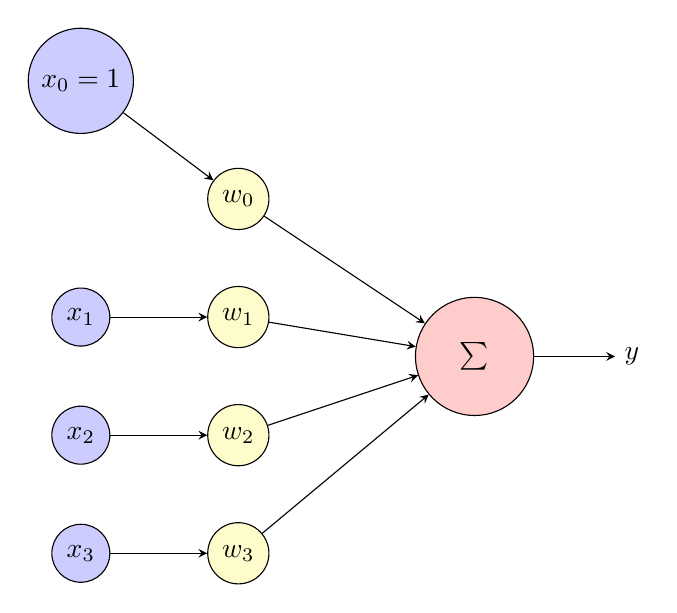
\begin{tikzpicture}[>=stealth]
    % Input nodes
    \node[draw, circle, fill=blue!20] (input0) at (0,4) {$x_0=1$}; % bias as input node
    \foreach \i in {1,2,3}
        \node[draw, circle, fill=blue!20] (input\i) at (0,2.5-\i*1.5) {$x_\i$};
        
    % Weight nodes
    \foreach \i in {0,...,3}
        \node[draw, circle, fill=yellow!20] (weight\i) at (2,2.5-\i*1.5) {$w_\i$};
        
    % Output node
    \node[draw, circle, fill=red!20, minimum size=1.5cm] (output) at (5,0.5) {$\sum$};
    
    % Output label node
    \node (outputLabel) at (7,0.5) {$y$};

    % Connections from input nodes to weight nodes
    \foreach \i in {0,...,3}
        \draw[->] (input\i) -- (weight\i);
    
    % Connections from weight nodes to output node
    \foreach \i in {0,...,3}
        \draw[->] (weight\i) -- (output);
    
    % Connection from output node to output label
    \draw[->] (output) -- (outputLabel) node[midway, above] {};
\end{tikzpicture}
\end{center}

    \caption{Visual diagram of a perceptron with bias term as $w_0$}
    \label{fig:perceptron}
\end{figure}

\subsection{Algorithm Overview} \label{def:PLA}
The Perceptron Learning Algorithm (PLA) is a binary classifier that attempts to find a separating hyperplane for data points. This hyperplane is determined by the weight vector \( \mathbf{w} \) and a bias \( b \). The algorithm iteratively adjusts the weights to classify the data points correctly.

\begin{figure}[H]
    \centering
    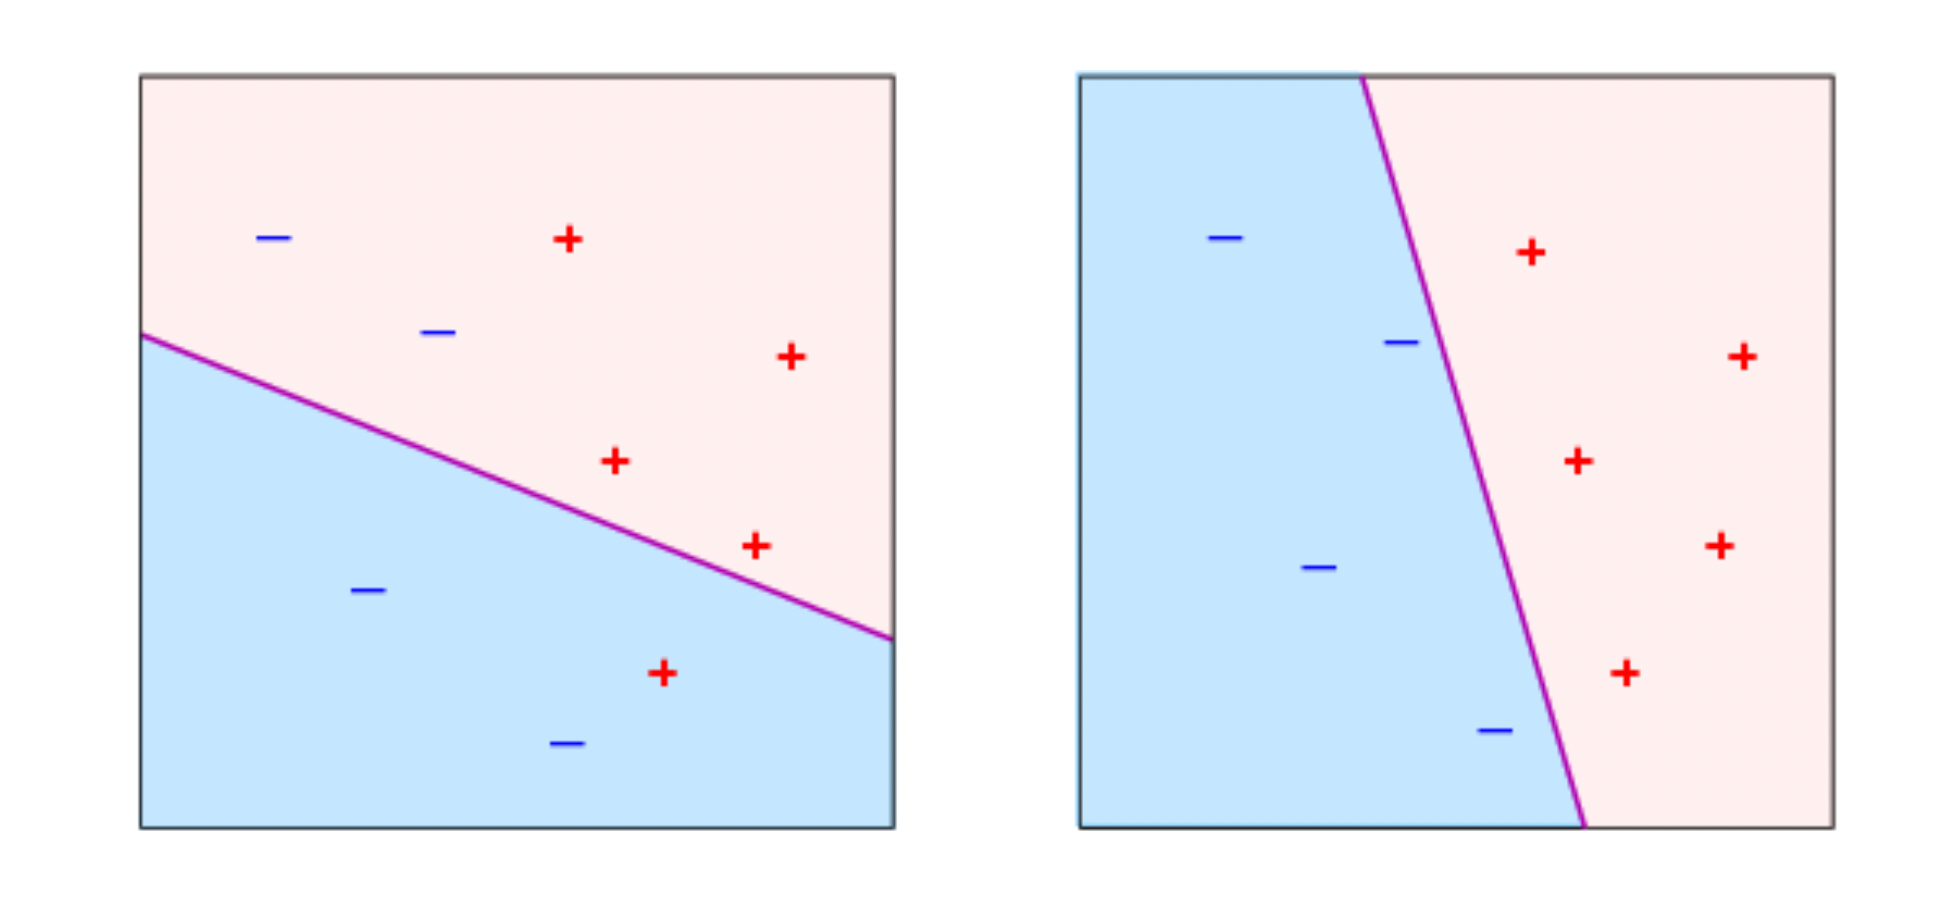
\includegraphics[width=0.5\textwidth]{img/pla-plot.png}
    \caption{Linearly Separable Data}
    \label{fig:pla-plot}
\end{figure}

\begin{definitionbox}{PLA Algorithm Steps}
    \begin{enumerate}
    \item \textbf{Initialisation}: Begin with a random weight vector \( \mathbf{w} \).
    \item \textbf{While there exists a misclassified data point}: 
    \begin{itemize}
        \item For \( y \in \{-1, +1\} \): If \( \text{sign}(\mathbf{w}^\top \textbf{x} _i) \neq y_i \) then update the weights:
        \[
        \mathbf{w} \leftarrow \mathbf{w} + y_i x_i
        \]

    \end{itemize}
    \item Repeat until all data points are correctly classified or a set number of iterations is reached.
\end{enumerate}

\end{definitionbox}



\subsection{Intuition}
\subsubsection{Visualising the Decision Boundary}
Imagine a 2D plane with two types of points: red and blue. The perceptron seeks a line where all red points lie on one side and all blue points on the other. The equation for such a line is:
\[ ax + by + c = 0 \]

\noindent
This can be represented more generally for higher dimensions as:
\[ \mathbf{w}^\top\mathbf{x} = 0 \]
where $\mathbf{w}$ is the weight vector and $\mathbf{x}$ is the input feature vector.


\noindent
Note that we do not specify a bias term, which for our 2D example, is the y-intercept.

\subsubsection{Learning with the Perceptron Algorithm}
Begin with an arbitrary weight vector $\mathbf{w}$. For each data point $\mathbf{x}_i$, the prediction $h(\mathbf{x}_i, \mathbf{w})$ is determined by the sign of $\mathbf{w}^T\mathbf{x}_i$. If this prediction aligns with the actual label $y_i$, no adjustments are made. Otherwise, the weights are updated to better classify the data point:
\[ \mathbf{w} \leftarrow \mathbf{w} + y_i\mathbf{x}_i \]

\subsubsection{Interpreting the Weight Vector}
The weight vector $\mathbf{w}$ sets the orientation of the separating hyperplane (or line, in 2D). It can be thought of as a vector perpendicular to this plane (or line, in 2D). The quantity $\mathbf{w}^T\mathbf{x}$ computes the position of point $\mathbf{x}$ relative to the origin, along the direction of $\mathbf{w}$. The sign indicates which side of the plane $\mathbf{x}$ lies on.\\

\noindent
When updating $\mathbf{w}$, the separating hyperplane shifts to better classify the misclassified data point $\mathbf{x}_i$.

\subsubsection{Equation for Weight Update}
To comprehend the weight update rule, consider the following equation:

\begin{align*}
y_i\cdot\mathbf{w}^{\prime\top}\mathbf{x}_i &= y_i\cdot(\mathbf{w}+y_i\mathbf{x}_i)^\top\mathbf{x}_i \\
&= y_i\cdot\mathbf{w}^\top\mathbf{x}_i + y_i^2\cdot\mathbf{x}_i^\top\mathbf{x}_i \\
&= y_i\cdot\mathbf{w}^\top\mathbf{x}_i + \|\mathbf{x}_i\|^2
\end{align*}

\begin{itemize}
    \item \( \mathbf{w'} \) is the updated weight vector after the weight adjustment rule has been applied. It is defined as \( \mathbf{w'} = \mathbf{w} + y_i\mathbf{x}_i \).
    \item The dot product \( \mathbf{w}^\top\mathbf{x}_i \) measures the alignment between the weight vector and the input feature vector. It gauges how close or far the point \( \mathbf{x}_i \) is from being correctly classified.
    \item The term \( y_i \) signifies the true class of the data point.
     \item \( y_i \cdot \mathbf{w}^\top\mathbf{x}_i \) is positive when the data point \( \mathbf{x}_i \) is correctly classified as the signs of  $\mathbf{w}^\top \mathbf{x}_i$ and $y_i$ match.
    \item \( y_i \cdot \mathbf{w}^\top\mathbf{x}_i \) is negative when the data point \( \mathbf{x}_i \) is misclassified  as the signs of  $\mathbf{w}^\top \mathbf{x}_i$ and $y_i$ do not match.
    \item If the point \( \mathbf{x}_i \) is misclassified, the weights need adjustment in the direction of \( y_i \mathbf{x}_i \). This term \( y_i\mathbf{x}_i \) acts as the corrective factor to guide the update. Remember, our goal is to have a positive  \( y_i \cdot \mathbf{w}^\top\mathbf{x}_i \) that is large (see next section on maximising the margin.)
    \item As \( y_i^2 \) is always positive (because \( y_i \) is either +1 or -1), the term \( \|\mathbf{x}_i\|^2 \) always has a positive contribution during the update, indicating that the magnitude of the feature vector plays a consistent role in the update.
    \item The updated weight vector \( \mathbf{w'} \) becomes more aligned with the misclassified point, improving future predictions.
    \item An animated diagram can be found \href{https://upload.wikimedia.org/wikipedia/commons/a/aa/Perceptron_training_without_bias.gif}{here}:

\end{itemize}


\subsection{Maximising the Margin}
The aim of the Perceptron is to maximise the margin by which points are classified. When adjusting the weight vector \( \mathbf{w} \) using a misclassified point \( x_i \), the updated weight vector \( \mathbf{w'} \) is more aligned with \( x_i \) in the direction of the correct label \( y_i \). This ensures that the product \( y_i \cdot \mathbf{w'}^T x_i \) becomes larger, leading to a more robust decision boundary with larger margins.

\subsection{Considering Bias}
So far we have considered instances of a 2D perceptron where every revision of the algorithm redraws a hyperplane line that passes through the origin. \\

\noindent
To consider the set of all possible hyperplanes in $\mathbb{R}^2$ is possible to redefine the hyperplane to be $\textbf{w}^\top \mathbf{x} + b = 0 $, so the hyperplane no longer has to pass through the origin, leaving us with a new algorithm.


\begin{enumerate}
    \item \textbf{Initialisation}: Begin with a random weight vector \( \mathbf{w} \) and bias \( b \).
    \item \textbf{While there exists a misclassified data point}: 
    \begin{itemize}
        \item For \( y \in \{-1, +1\} \): If \( \text{sign}(\mathbf{w}^\top \textbf{x} _i + b) \neq y_i \) then update the weights:
        \[
        \mathbf{w} \leftarrow \mathbf{w} + y_i x_i
        \]

        \item And update the bias:
        \[ b' = b + y_i \]

    \end{itemize}
    \item Repeat until all data points are correctly classified or a set number of iterations is reached.
\end{enumerate}

\noindent
To simplify computation, we can implement bias as part of $\textbf{w}$ by increasing the dimensions of $\textbf{w}$ by one, and setting $x_0$ to 1 and $w_0$ to the bias. Then we use the algorithm in \ref{def:PLA}




\subsection{Remarks}
The Perceptron Learning Algorithm will stop after a finite number of iterations if the data is linearly separable. Otherwise, it requires an external stopping condition, such as a predefined maximum number of iterations, or it chooses the hyperplane with minimal misclassification errors (Pocket Algorithm)

\section{Linear Regression}
Linear regression is a supervised learning algorithm primarily used for modelling the relationship between a scalar dependent variable and one or more independent variables. In the context of classification, linear regression can be applied to predict continuous values which are then thresholded to produce discrete class labels.

\subsection{Regression Error}
Given a dataset with $n$ samples, the regression error $\hat{R}_n(h)$ is defined as the average squared difference between the predicted and actual values:

\begin{align}
    \hat{R}_n(h) &= \frac{1}{n} \sum_{i=0}^{n} (h(\textbf{w}, \textbf{x}_i) - y_i)^2 \\
    \hat{R}_n(\textbf{w}) &= \frac{1}{n} \sum_{i=0}^{n} (\textbf{w}^\top \textbf{x}_i - y_i)^2 \\ \label{eq:regerror}
    &= \frac{1}{n} ||X\textbf{w} - \textbf{y}||^2
\end{align}

where:
\begin{itemize}
    \item $X$ is the data matrix where each row $x_i^T$ represents a sample.
    \item $y$ is the label vector.
\end{itemize}

\subsection{Closed-Form Solution (Least-Squares)}
The optimal weight vector $w$ that minimises the regression error can be found by setting the gradient of $\hat{R}_n(w)$ to zero:

\begin{align*}
    \nabla \hat{R}_n(w) &= 0 \\
    \begin{aligned}
        &\text{From \eqref{eq:regerror} we differentiate} \\
        &\frac{2}{n}X^\top(X\textbf{w} - \textbf{y}) = 0 \\
        &X^\top X\textbf{w} = X^\top \textbf{y}
    \end{aligned}
\end{align*}

\begin{definitionbox}{Closed-Form Solution for Least-Squares}
From the above, the solution for $\textbf{w}$ is:

$$
    \textbf{w} = (X^\top X)^{-1} X^\top \textbf{y}
$$
    
\end{definitionbox}


Here, $(X^\top X)^{-1} X^\top$ is known as the Moore-Penrose pseudoinverse of $X$. 

\subsection{Classifier Thresholding}
Once $\textbf{w}$ is found, predictions can be made for new data points. In the context of classification, the predicted continuous values can be thresholded (e.g., at 0.5 for binary classification) to produce discrete class labels.








